\documentclass[12pt]{article}

\usepackage{sbc-template}
\usepackage{graphicx,url}
\usepackage[utf8]{inputenc}
\usepackage[brazil]{babel}
\usepackage{float}

\usepackage{indentfirst} % SBC nao usa indentfirst, mas acho melhor com identacao

\title{Estudo de Caso de Solução Agnóstica para Gerenciamento de Recursos em Multi-nuvem}

\author{Alexandre Canalle\inst{1}, Ariel Frozza\inst{1}}

\address{Departamento de Informática -- Pontifícia Universidade Católica do Paraná (PUC-PR)\\
	Caixa Postal 15.064 -- 91.501-970 -- Curitiba -- PR -- Brazil
	\email{arielfrozza@gmail.com, roxsnd@gmail.com}
}

\begin{document}

\sloppy
\maketitle
	
\begin{abstract}
	This meta-paper describes the style to be used in articles and short papers
	for SBC conferences. For papers in English, you should add just an abstract
	while for the papers in Portuguese, we also ask for an abstract in
	Portuguese (``resumo''). In both cases, abstracts should not have more than
	10 lines and must be in the first page of the paper.
\end{abstract}

\begin{resumo} 
	Este artigo explora os conceitos de Multi-nuvem e Infraestrutura como Código.Também são descritas as dificuldades na interoperabilidade entre múltiplos provedores de Nuvem e serão discutidas possíveis soluções para as dificuldades descritas. Por fim, será apresentado um caso de uso da ferramenta Terraform para implementação de um serviço WEB em duas Nuvens distintas (AWS e Openstack), com intuito de verificar a efetividade de uma solução agnóstica para gerenciamento de Multi-nuvem.
\end{resumo}

	\section{Introdução}
	    Atualmente, o uso simultâneo de serviços e recursos de múltiplos provedores de Nuvem é justificado pela necessidade de seus consumidores, expressas em requerimentos tais como qualidade de serviço e custo. As organizações que estão migrando para a Nuvem, seja para estender ou substituir sua infraestrutura \textit{on-premises}, buscam soluções confiáveis, seguras e, se possível, sem aprisionamento à fornecedores ou soluções fechadas (\textit{vendor lock in}).
	    
	    Este estudo de caso discute princípios, conceitos e desafios e apresenta algumas ferramentas envolvidas no uso simultâneo de recursos de múltiplos provedores de Nuvem (Públicas ou Privadas). Também serão levantados alguns dos principais pontos de atenção na utilização das atuais soluções que se propõem a gerenciar recursos de IaaS ou PaaS de múltiplas Nuvens. O cenário ideal seria poder utilizar uma solução (software) que possa gerenciar múltiplas Nuvens de forma centralizada, onde uma única instrução de código possa criar recursos de IaaS ou Paas em diferentes provedores. Há poucas soluções agnósticas (Open source ou proprietárias) disponíveis no mercado, já que, as APIs das principais Nuvens diferem muito entre si, dificultando o aproveitamento de código.
	    
	    Conceitos relevantes para o tema, tais como Infraestrutura como Código, a definição e os benefícios do uso de um ambiente em Multi-nuvem são discutidos primeiramente. Em seguida, um modelo padrão de arquitetura para Multi-nuvem é apresentado. A partir dessa arquitetura de referência, algumas soluções (software) que tornam possíveis a Infraestrutura como Código em Multi-nuvem são apresentados e discutidos. Por fim, será feita uma experimentação disponível em https://github.com/arielfrozza/multi-cloud destacando os processos, requisitos e desafios na implementação de IaaS em Multi-nuvem usando uma ferramenta Opensource, o Terraform. O estudo será realizado à luz dos princípios da Infraestrutura como Código, validando em que condições os códigos podem ser reaproveitados, e também, se há vantagens no uso desta solução, frente às soluções fechadas de cada provedor de Nuvem.
		
	\section{Definição e Necessidade de Multi-nuvens}
	
	Diferentes provedores de Nuvem podem ser usados de forma combinada para atender às necessidades de negócio de empresas, onde o conjunto de infraestruturas distribuídas pode ser definido e gerido como código, ao utilizar conceitos e ferramentas próprias do desenvolvimento de software. A seguir serão apresentados os conceitos de Multi-nuvem e Infraestrutura como Código, bem como algumas motivações para uso de múltiplos provedores de Nuvem.
	
	\subsection{Definição de Multi-nuvem}
	
	Muitos termos são encontrados na literatura para designar o uso simultâneo de duas ou mais Nuvens. A citar os mais recorrentes \cite{Ferrer:2012}; \textit{Multi-cloud, Cloud-federation, Inter-cloud, Hybryd Cloud, Cloud of Clouds, Sky Computing, Aggregated Clouds, Fog Computing} e \textit{Distributed Clouds}. Sendo assim, torna-se útil delimitar o conceito de Multi-nuvem abordado neste artigo de outros modelos de uso combinado de Nuvens.
	
	De acordo com \cite{Ferrer:2012}, existem dois modelos de entrega de serviços em múltiplas Nuvens; Nuvem Federada e Multi-nuvem (\textit{Federated Cloud} e \textit{Multi-Cloud}). A diferença entre estes modelos seria o grau de colaboração entre os provedores de Nuvem e pelo modo com o qual os usuários interagem com as Nuvens. No primeiro modelo há o acordo de uso compartilhado dos recursos entre os provedores. Os usuários de uma Nuvem federada não ficam sabendo, na maioria dos casos, de qual dos provedores um determinado recurso está sendo consumido. No caso do Multi-nuvem, o usuário está ciente e é responsável pela alocação de recursos em um ou outro provedor e não há anuência dos provedores para uso compartilhado de recursos entre os provedores.
	
	\textit{Sky Computing, Aggregated Clouds, Multi-tier Clouds} ou \textit{Cross-Cloud} são casos particulares de Nuvens Federadas e portanto não serão abordadas neste artigo. 
	
	O tipo mais comum de Multi-nuvem é o híbrido, que envolve duas ou mais Nuvens, por exemplo, uma Privada e uma Pública. Comumente, esse modelo híbrido é usado para transbordo de capacidade (\textit{cloud bursting}) onde os recursos são expandidos para a Nuvem Pública quando os recursos da Nuvem Privada chegam nos níveis máximos pré-definidos \cite{Ferrer:2012}. A migração de uma Nuvem para outra, mesmo que apenas uma vez, é outro exemplo de uso de Multi-nuvem.
	
	A interoperabilidade entre os diversos serviços ofertados e orquestração de recursos em múltiplas Nuvens (usando Infraestrutura como Código \cite{Morris:2016}, por exemplo) ainda está distante da maturidade. De acordo com \cite{Fisher:2018}, todos os provedores de Nuvens experimentam, eventualmente, períodos de indisponibilidade que podem causar impactos a negócios. Também pode ser um problema a performance variável quando os provedores de Nuvem fazem a oversubscrição (\textit{overprovision}) da sua infraestrutura virtualizada e isto resulta em degradação de performance e qualidade de serviço \cite{CloudSpectator:2017}. Outro ponto importante é que a maioria dos provedores de Nuvem  (inclusive os líderes de mercado) disponibilizam Software e APIs proprietárias, que não são aderentes à padrões de \textit{Cloud API} como propostos por OASIS TOSCA \cite{TOSCA:2019} ou OASIS CAMP \cite{CAMP:2019}.
	
	\subsection{Infraestrutura como Código}
	
	Infraestrutura como código – IaC (\textit{Infrastructure as Code}) é o processo de gerenciamento e provisionamento de recursos de infraestrutura através de código e arquivos de configuração que descrevem o estado desejado para os recursos de infraestrutura. IaC usa definições declarativas ao invés de processos manuais ou procedurais. Como se tratam de arquivos de código, as definições podem ser armazenadas em um sistema de controle de versões, tal como o Git.
	 
	Algumas vantagens da utilização de IaC incluem a eliminação de tarefas repetitivas possibilitando a fácil replicação de implementações, quando o bloco de código pode ser executado repetidas vezes, fazendo poucas modificações. Por exemplo, para criar ou modificar recursos em diferentes ambientes (Produção, Teste, Desenvolvimento) Nuvens (GCP, Azure ou AWS por exemplo). Uma vez que a infraestrutura  está codificada de forma estruturada e geralmente em módulos, o código pode ser reaproveitado. O fato do código que define a infraestrutura, estar versionado em ferramentas como Git, possibilita maior controle nas aplicações de mudança nos ambientes facilitando, inclusive, a recuperação de desastres. Essa característica também possibilita a simplificação da documentação do código, bem como sua manutenção e suporte. Além disso, com IaC, fica fácil utilizar-se das mesmas técnicas de planejamento e testes automatizados há muito tempo utilizadas por desenvolvedores.	
	
	\subsection{Motivações para Uso de Multi-nuvens}
	
	Os motivos que justificam o uso de múltiplas Nuvens são inúmeros e dependem da natureza do negócio de cada usuário, mesmo assim é possível citar algumas vantagens do uso simultâneo de dois ou mais provedores de Nuvem:
	
	\textbf{Tolerância à falhas} (\textit{fault-tolerance}) ao envolver uso de mais de um provedor de Nuvem simultaneamente, permitindo movimentações de contingência no caso de indisponibilidade de um dos provedores, por exemplo.
	
	\textbf{Neutralidade de fornecedor} possibilita a implementação de IaaS e/ou PaaS nos principais provedores de Nuvens usando soluções diversas (em especial \textit{open-source}) evitando o aprisionamento à um fornecedor (\textit{vendor lock-in}).
	
	\textbf{Performance} ao possibilitar ajustes nos níveis de carga para outros provedores de Nuvem em caso de degradação de performance ou qualidade de serviço em um dos provedores.
	
	\textbf{Segurança} ao possibilitar a fácil migração de serviços para provedores mais aderentes aos parões de segurança exigidos pela natureza do serviço ofertado.
	
	\textbf{Eficiência de custos} como habilidade de aproveitar os melhores preços de recursos computacionais e serviços em um ambiente Nulti-nuvem.
	
	Os custos de operação dos provedores de Nuvem variam em função dos requisitos de uso e da época de contratação dos serviços. Desta forma, os custos de trocar de provedor podem ficar muito altos caso a infraestrutura e/ou aplicações tenham que ser refeitas inteiramente. Por exemplo, um dos modelos de compra de VMs da Amazon, o AWS Spot Instance, oferece descontos para certos casos de uso, que podem chegar a 90\%, quando sua infraestrutura encontra-se ociosa. Outro exemplo é reflexo da redução dos custos operacionais dos provedores de Nuvem ao longo do tempo. De 2011 para 2013, o custo por hora do AWS EC2 baixou cerca de 30\% \cite{Golden:2013}. Com o uso de padrões \textit{vendor neutral}, o objetivo seria possibilitara troca de provedor ou priorizar a execução \textit{on-premises} de acordo com a conveniência, sem ter que alterar o \textit{software stack}.
	
	A seguir será descrito um \textit{framework} para o uso de Multi-nuvem envolvendo duas Nuvens, uma Privada e outra Pública. 
	
	\section{Arquitetura de Referência para Multi-nuvem}
	
	Conforme ilustrado na Figura~\ref{fig:figure1}, será explorado um padrão de implementação de Multi-nuvem que propõem ajudar a atender alguns casos comuns de uso:
	
	\textbf{Transbordo para Nuvem Pública} (\textit{Bursting Pattern}): em algumas situações, a capacidade \textit{on-premises} de uma empresa pode exaurir e pode-se querer usar a capacidade em uma Nuvem pública para suprir uma determinada demanda.
	
	\textbf{Alta Disponibilidade}: eventualmente, um provedor de Nuvem pode ficar (parcial ou totalmente) indisponível ou com degradação na qualidade dos serviços por diversos motivos. Pode-se querer migrar de um provedor para outro os serviços e recursos para não impactar o usuário final. Por exemplo, em caso de falha ou manutenção do Data Center que hospeda a Nuvem privada, migram-se os serviços para uma Nuvem pública, mesmo que temporariamente.
	   
	\textbf{Eficiência de Custos}: em alguns casos, provedores oferecem descontos ou modificam seus preços em função da oferta e demanda, possibilitando transferência de recursos e serviços de uma Nuvem para outra sem que o usuário final seja impactado.
	
	A Figura~\ref{fig:figure1} ilustra as atividades e processos envolvidos para atingir os objetivos descritos acima. Outros benefícios, tais como Tolerância à Falhas, Segurança, Validação experimental, etc, também podem ser alcançados usando este mesmo padrão ou após serem feitas pequenas modificações, os quais não serão diretamente abordados neste artigo, mas podem ser entendidos de forma mais completa em \cite{Fisher:2018}.
	
	Está numerada na Figura~\ref{fig:figure1} a ordem do processo de provisionamento de recursos em Multi-nuvem, que inicia em \textbf{Multi-cloud Telemetry (1)} com a coleta e agregação de dados de capacidade das Nuvens integrantes da infraestrutura. Na Figura~\ref{fig:figure1} estão representadas uma Nuvem Privada e outra Pública, mas é possível expandir essa mesma arquitetura para um conjunto maior de diferentes provedores. As informações coletadas são repassadas para o \textbf{SLA Enforcer Rules Engine}, que valida a condição para a migração de recursos de uma Nuvem para outra. Por exemplo, se a capacidade de uma das Nuvens chegar a 80\%, faz-se deploy de novos recursos apenas na outra Nuvem. O \textbf{SLA Enforcer Rules Engine} avalia um conjunto de condições que se faça adequado para cada negócio ou situação, validando condições de custo ou tempo de resposta, além da capacidade. O resultado deste processo dispara o gatilho para iniciar as novas implementações através do \textbf{Multi-nuvem Deployer/Orquestrator}. Além disso, o \textbf{Multi-nuvem Telemetry \& Log Aggregator}, também gera subsídio para a bilhetagem através de métricas de utilização que são contabilizadas e disponibilizadas para o usuário através do processo \textbf{Multi-cloud Billing}. Também os alertas de erros são tratados e processados pelo \textbf{Sistema de Alertas e Notificações}.
		
	\begin{figure}[H]
		\centering
		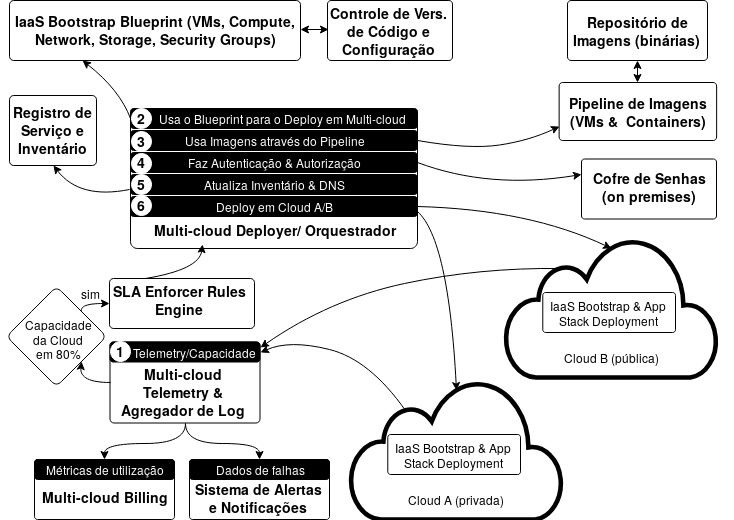
\includegraphics[width=0.9\linewidth]{figuras/Figure1.png}
		\caption{Diagrama de relacionamentos de processos em Multi-nuvem.}
		\label{fig:figure1}
	\end{figure}

	 As etapas \textbf{(2)} e \textbf{(3)} do processo \textbf{Multi-nuvem Deployer/Orquestrator} utilizam as definições de implementações armazenadas como código em texto em controle de versão(Git, por exemplo). Estas definições de implementações são aplicadas sobre as imagens selecionadas do \textbf{Pipeline de Imagens} que podem ser VMs (em formato OVA, VMDK, VHD ou RAW) ou Containers (Docker, por exemplo).
	
	Toda informação sensível, em especial senhas ou chaves são obtidas do \textbf{Cofre de Senhas} \textbf{(4)}, que por motivos de segurança e de facilidade de acesso, geralmente está \textit{on-premises} e não em uma das Nuvens que fazem parte da Multi-nuvem.   
	
	Os serviços e itens de configuração ativos são registrados no \textbf{Registro de Serviços e Inventário (5)}, bem como o DNS é atualizado para refletir os novos registros e rotas.
	
	Alguns processos do \textbf{Cloud Deployer/Orquestrator (6)} criam os componentes, que foram definidos nas etapas anteriores, em cada uma das Nuvens especificadas usando as APIs de cada fornecedor. Os softwares usados nesta etapa do Cloud Deployer devem possuir uma camada de abstração das diversas APIs para que a implementação seja o mais transparente possível e que os códigos envolvidos possam ser reaproveitados e não sejam complexos, ou difíceis de manter e documentar (alguns softwares serão apresentados e demonstrados na seção a seguir).  

	O cenário descrito acima inicia em \textbf{Telemetry (1)}, assim possibilitando situações automatizadas de orquestração dos recursos na Multi-nuvem, entretanto, um humano também poderia iniciar esse processo, passando instruções diretamente ao \textbf{Multi-cloud Deployer/Orquestrator}.  
	
	Os processos descritos acima e esquematizados na Figura~\ref{fig:figure1} podem ser bastante complexos, envolver outros subprocessos e também um conjunto diversificado de ferramentas e softwares. Como exemplo, será explorado em mais detalhes o \textbf{Pipeline de Imagens}.
		
	\begin{figure}[ht]
		\centering
		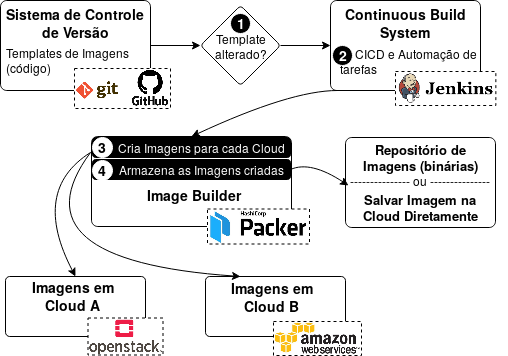
\includegraphics[width=0.7\linewidth]{figuras/Figure2.png}
		\caption{Diagrama do processo de Pipeline de Imagens.}
		\label{fig:figure2}
	\end{figure}
    
	O objetivo do processo da Figura~\ref{fig:figure2} é prover imagens binárias padronizadas de servidores que estão dentro dos padrões para rodar em qualquer Nuvem IaaS que fazem parte da Multi-nuvem. Para alcançar seus objetivos, este processo utiliza produtos \textit{open-source}. Os referenciados na Figura~\ref{fig:figure2} são; \textbf{Packer} (https://www.packer.io) que é um framework capaz de produzir múltiplas imagens em formatos diferentes, apropriadas para a maioria dor provedores de Nuvem (Públicas e Privadas). Packer pode ser usado com uma variedade grande de \textit{build systems}, dentre os quais destacamos o \textbf{Jenkins} (https://jenkins.io), que é uma plataforma para entrega contínua (\textit{Continuous Delivery}) de \textit{releases} de software em ambiente distribuído.

	O processo ilustrado na Figura~\ref{fig:figure2} é iniciado a partir de um \textit{commit} no \textbf{Sistema de Controle de Versão} em alguma \textit{branch} (Master por exemplo) que é monitorada pelo \textbf{Continuous Build System (1)}. Sempre que uma alteração é feita, o Jenkins executa as rotinas \textbf{(2)} que são requisitos para que o Packer (principal software do \textbf{Image Builder}) possa gerar as imagens de acordo com os \textit{blueprints} de cada Nuvem \textbf{(3)}. O Packer pode armazenar essas imagens para uso futuro em um repositório centralizado (\textit{on-premises} geralmente) ou pode também gravar cada imagem na respectiva Nuvem \textbf{(4)}, essa última alternativa pode ser mais rápida na hora de criar uma instância, pois não precisa fazer a transferência (via Internet) da Imagem armazenada \textit{on-premises} para a Nuvem.
	
	\section{Validação Experimental - \textit{Deployment} de aplicação em Multi-nuvem}
	
	Uma das maneiras de experimentar e explorar o processo de \textit{deploy} de IaaS ou PaaS em Multi-nuvem pode ser feito através do uso de alguns softwares que automatizam a criação de recursos em Nuvem. O uso das consoles WEB ou outros mecanismos disponibilizadas pelos principais provedores de Nuvem, podem ser usados para alguns casos de uso, mas, de forma geral,  propiciam maior chance de erro humano, requerem que a documentação seja feita adicionalmente (geralmente nas fases conclusivas dos projetos) e não aproveitam os benefícios da Infraestrutura como Código (IaC), discutidos anteriormente.
	
	Existem diversas ferramentas que trabalham sob o conceito de IaC e que atendem os requisitos para criação de infraestrutura em Multi-nuvem, uma delas um serviço nativo do Openstack, o Heat, que interage com a API do Openstack para criação ou modificação de Infraestrutura. Heat também consegue atuar em AWS, mas alguns recursos de Infraestrutura ainda não estão definidos no Heat, e, portanto o seu escopo de atuação, para AWS especificamente ainda é muito restritivo, fazendo com que ele não seja usado em ambientes de produção corporativos. 
	
	Outras ferramentas, tais como Chef, Puppet, Ansible e SaltStack que são muito utilizadas, inclusive em ambientes produtivos, para gerenciamento de configuração de servidores também podem ser usados para criação de recursos e infraestrutura em Nuvens públicas ou Privadas. Estes softwares, entretanto, dependem de módulos, bibliotecas ou outros softwares adicionais para interagirem com as APIs das diversas nuvens suportadas por essas ferramentas. Outro fator limitante é que, nuvens com menor expressividade no mercado tendem a ter menor suporte por parte dessas ferramentas.
	
	Há ainda outra forma de interagir com as APIs das Nuvens, que é via Software Development Kit - SDK (por exemplo, a AWS utiliza boto3, em Python) e cada provedor de Nuvem disponibiliza seu próprio SDK e eles geralmente diferem muito entre si, o que implica que o SDK de uma Nuvem não pode ser usado em outra.
	
	Das soluções listadas acima, podemos notar algumas características que podem ser limitações para uso em produção em ambientes de Multi-nuvem. Os SDKs da maioria dos provedores de Nuvem atende apenas as especificações de API do respectivo provedor de Nuvem (assim como outras ferramentas, como o CloudFormation, que atende somente AWS) e portanto não são boas soluções para gerenciar Multi-nuvem com IaC, pois, não favorecem a fácil replicação de implementações, o reaproveitamento de código, bem como sua manutenção e suporte. Como descrito anteriormente, a maioria dos provedores de Nuvem não oferecem APIs padronizadas, dificultando muito o desenvolvimento de ferramentas agnósticas. As ferramentas como Chef, Puppet, Ansible e SaltStack têm foco no gerenciamento de configuração de servidores e não oferecem bom suporte e escopo para criação de infra em múltiplos provedores de Nuvem \cite{Morris:2016}.
	
	Para gerenciar múltiplas Nuvens simultaneamente, é preciso que o Software possa interagir com as diversas APIs dos provedores de Nuvens (públicas ou privadas) e que conte com suporte o mais amplo possível ao gerenciamento dos recursos das Nuvens. Além disso, é importante que a solução tenha constante manutenção e atualizações, em especial a inclusão (rápida) das novas funcionalidades ou serviços que os provedores venham a lançar. Esta característica pode ser medida pela atividade e quantidade de contribuidores do GitHub, por exemplo (e eventualmente usada como critério de comparação com outras ferramentas). De forma complementar, pode-se desejar que a ferramenta tenha uma estrutura de suporte técnico formal (pago) para atender à necessidade (eventualmente regulatória) de algumas corporações.
	
	Durante a pesquisa para este estudo de caso, identificou-se o Terraform, que é uma solução open-source específica para a criação de infraestrutura em Nuvem (dentro do modelo IaC), como uma promissora possibilidade para atender os principais requisitos descritos anteriormente. Diferentemente de ferramentas como o CloudFormation ou os SDKs, o Terraform é uma solução agnóstica, permitindo-lhe criar infraestrutura em praticamente qualquer ambiente, seja ele em Nuvem (Amazon AWS, Microsoft Azure, Google GCP, IBM Cloud, Digital Ocean, etc.), ambiente virtualizado, local ou em Data Centers (VMWare, Xen, Virtual Box, etc.), Docker, Kubernetes, além de recursos diversos de infraestrutura e softwares, tais como Redes (F5 BIG-IP, Palo Alto Networks, etc.), bancos de dados (MySQl ou PostgreSQL), dentre outras (ver www.terraform.io). Terraform conta com uma sólida e ativa comunidade de contribuidores (https://github.com/hashicorp/terraform) e a Hashicorp, empresa que criou o Terraform, oferece suporte, consultorias e treinamento com foco no mercado corporativo.
	
	Na seção a seguir utiliza-se o Terraform para fazer o provisionamento de um servidor com uma aplicação web de teste em duas Nuvens; Openstack e AWS, com o intuito de verificar se o código desenvolvido para os dois provedores atende aos requisitos e características da IaC, conforme listados e discutidos anteriormente.  
	
	\subsection{Validação Experimental com Terraform}
		
	Em https://github.com/arielfrozza/multi-cloud estão disponibilizados os arquivos de código que foram utilizados para a experimentação deste estudo de caso, e que fazem o \textit{deploy} de uma aplicação WEB simples em duas nuvens diferentes; AWS e Openstack. Esse cenário tem o objetivo de representar o uso de um caso particular de Multi-nuvem, que é a Nuvem híbrida. A execução desses códigos pode ser feita mediante instalação do Terraform em \textit{host} com acesso às duas Nuvens, e deve-se ter também as credenciais necessárias para a criação de instâncias. Os detalhes dos códigos e sua implementação não serão descritos neste artigo, mas os detalhes e passo a passo encontram-se no repositório do GitHub abaixo dos diretórios openstack\_tf e aws\_tf, para cada uma das duas Nuvens.
	
	O Terraform utiliza como \textit{input} um conjunto de arquivos contendo a definição da infraestrutura, escrita em uma linguagem própria do Terraform, a ser criada nas duas Nuvens. A arquitetura dessa validação segue o modelo apresentado na Figura~\ref{fig:figure1}, mas não de forma integral. O interesse deste estudo é apenas verificar e identificar as vantagens e também as limitações do uso de tal solução à luz dos conceitos de IaC definidos anteriormente. Para tal, é criada uma instância Ubuntu 18.04 em cada uma das Nuvens seguido de instalação de alguns softwares (Python 2.7 e Flask) e \textit{deploy} de um código HTTP REST simples (escrito em Flask).
	
	Desta forma, não serão abordadas nem discutidas as etapas de Telemetria	(e as métricas ou SLAs envolvidos), Pipeline de Imagens, Cofre de Senhas ou Registro de Serviço e Inventário. Processos indicados pelos números 1, 3, 4, 5 na Figura~\ref{fig:figure1}.
	
	A estrutura de código do Terraform (conforme documentada em www.terraform.io/guides) é bem estruturada e pode ser segmentada, permitindo que o código seja dividido em múltiplos arquivos para melhor organização e manutenção. 
	
	A Figura~\ref{fig:figure3a} lista os arquivos utilizados para este estudo e que estão disponíveis no GitHub. Os arquivos de extensão ".tf" e ".tfvars" contém o código Terraform que interage com as Nuvens para a execução das rotinas. Consta ainda, nestes diretórios, a aplicação de teste, em Flask (simple\_app.py) e o par de chaves (mykey e mykey.pub) para a conexão remota via SSH com as instâncias criadas nas duas Nuvens.  
	
	\begin{figure}[ht]
		\centering
		
\includegraphics[width=0.42\linewidth]{figuras/Figure3a.png}
		\caption{Comparativo da estrutura dos diretórios e listagem de arquivos das duas Nuvens.}
		\label{fig:figure3a}
	\end{figure}
	
	É importante, do ponto de vista da IaC, que os dois diretórios ilustrados na Figura~\ref{fig:figure3a} tenham a mesma estrutura e relação de arquivos, pois facilita a criação e atualizações de documentação e procedimentos operacionais. Além disso, possibilita o reaproveitamento de estruturas inteiras ou de blocos de código, a manutenção e o controle de versões e mudanças fica facilitado com a segmentação em diferentes arquivos com funções melhor definidas. 
	
	Entretanto, ao fazer a comparação do conteúdo de cada arquivo do Terraform (os ".ft"), é possível observar facilmente que os códigos diferem substancialmente, conforme ilustrado nas Figura~\ref{fig:figure3b} e Figura~\ref{fig:figure3}. Apesar da estrutura e quantidades de arquivos de código escritos para as duas Nuvens serem iguais, devido ao funcionamento do Terraform, a sintaxe para a criação de recursos pode mudar bastante dependendo do provedor de Nuvem em uso. Por exemplo, os métodos de autenticação são essencialmente diferentes para as duas Nuvens utilizadas neste estudo. O Openstack requer um usuário com senha e também a URL do Keystone, a região e o domínio utilizado, já a AWS requer apenas a chave de acesso e a \textit{secret key} para fazer a autenticação e autorização, conforme ilustrado na Figura~\ref{fig:figure3b}. 
		
	\begin{figure}[H]
		\centering
		
\includegraphics[width=0.8\linewidth]{figuras/Figure3b.png}
		\caption{Comparativo de código dos arquivos provider.tf para as duas Nuvens.}
		\label{fig:figure3b}
	\end{figure}
	
	Outro exemplo dessa diferença de sintaxe também pode ser observada na Figura~\ref{fig:figure3} em que apenas um trecho do código que provisiona as VMs é exibido, mas que mostra claramente que as instruções do Terraform para as duas Nuvens em estudo, diferem muito entre si.
	
	Essas diferenças entre as sintaxes do Terraform para cada provedor de Nuvem, acabou causando que todos os arquivos diferissem, no conteúdo, parcialmente de uma Nuvem para outra, conforme Figura~\ref{fig:figure3}. Este fato potencialmente dificulta o controle das mudanças de código e também o reuso de trechos quando, por exemplo, deseja-se replicar a infraestrutura em questão, para um terceiro provedor.
		
	\begin{figure}[ht]
		\centering
		
\includegraphics[width=0.97\linewidth]{figuras/Figure3.png}
		\caption{Comparativo de trecho de código dos arquivos instance.tf para as duas Nuvens.}
		\label{fig:figure3}
	\end{figure}

	Durante o desenvolvimento dos códigos em Terraform, foi possível obter grandes vantagens com o uso do GitHub para controle de versões no código, pois, cada mudança no código ou incremento, pode ser testado com mais frequência. Também a documentação ficou mas robusta e coerente, pois, a cada novo \textit{commit} feito no GitHub, as anotações de comentário eram obrigatórias e síncronas. O reúso de código também é facilitado quando um versionador de arquivos é usado. No caso do GitHub, um \textit{fork} poderia ser criado para o gerenciamento de infraestrutura ou configuração em outra Nuvem ou para a replicação em um ciclo de vida de aplicação; de Desenvolvimento para Homologação, que por fim pode ser promovido para Produção.
	
	No caso de haver interesse na replicação de uma implementação para um terceiro, ou vários outros, provedor(es) de Nuvem (por exemplo GCP, Azure, BlueMix, Mirantis, etc.) teriam apenas que ser incluídas ou retiradas algumas linhas específicas para aquela Nuvem e seriam alteradas também os valores e nomes das variáveis. Toda a estrutura, relação e quantidade de arquivos permaneceria igual às outras. Portanto, o reuso de código, mesmo que demandando um certo nível de esforço, pode ainda ser feito. 
	
	O Terraform também mostrou-se muito eficaz em abstrair para o usuário, as APIs das duas Nuvens estudadas. Em nenhuma etapa da escrita ou execução dos códigos foi necessário interagir ou escrever código que interagisse diretamente com as APIs das Nuvens em estudo. Isso facilita a escrita e documentação dos códigos.
	
	No caso de uso das SDKs (ou outros serviços como Heat e CloudFormation) das Nuvens, todo o código para interagir com as APIs das Nuvens seriam totalmente diferentes entre si, e nada poderia ser reaproveitado nos casos de extensão de serviços para um provedor de Nuvem adicional (e diferente das demais). 		
	
	\section{Conclusão}
	
	Multi-nuvem está sendo cada vez mais utilizada em ambientes corporativos, especialmente no formato de Nuvem híbrida, sendo uma ótima solução para que elas possam ofertar serviços WEB tolerantes à falhas, com ótima performance e com custos eficientes. A concorrência em alguns setores de serviços WEB e a crescente exigência do usuário por serviços rápidos, disponíveis e baratos, também pode impulsionar ainda mais o uso de Multi-nuvem. Porém, ainda há pouca disponibilidade de soluções agnósticas, completas e robustas o bastante no mercado, capazes de gerenciar recursos em diversos provedores de Nuvem Pública ou Privadas simultaneamente, de forma a atender as necessidades de gerenciamento de infraestrutura em Nuvem de tais empresas.
	
	Os principais provedores de Nuvem parecem se proteger do mercado Multi-nuvem ao criarem suas APIs de forma fechada. A não adesão a padrões de Nuvem API, como as propostas por OASIS \cite{CAMP:2019} (à qual o OpenStak é uma das poucas aderentes) torna muito difícil o desenvolvimento de soluções agnósticas que se propõem a resolver o problema do gerenciamento de recursos e infraestrutura em Multi-nuvem.
		
	Durante a validação experimental deste estudo, identificou-se o Terraform como uma das mais completas e robustas soluções para o caso, por ser uma solução agnóstica, desenvolvida para possibilitar o uso sob os princípios da Infraestrutura como Código, onde o versionamento (em GitHub neste estudo) e o reaproveitamento de código são valores importantes. O Terraform facilita o estabelecimento de processos padronizados e estruturados de desenvolvimento de código, por conseguir abstrair para o usuário, as APIs dos diferentes provedores de Nuvem. Idealmente, o usuário deveria poder trabalhar e manter apenas um código que pudesse provisionar em diversas Nuvens, entretanto, foi possível identificar que os códigos do Terraform apresentam substanciais diferenças de um provedor para outro, o que dificulta o reaproveitamento de código. 
	
	Apesar das limitações com relação ao reaproveitamento de código, o Terraform pode ser mais eficiente e eficaz que o uso de SDKs ou outras soluções, como Heat ou CloudFormation, por serem muito específicas para determinados provedores de Nuvem. Característica que impossibilita totalmente o reaproveitamento de código, bem como a replicação ou migração de implementações entre provedores de Nuvem diferentes. Em particular, no caso de uso para Multi-nuvem com grande número de provedores participantes, o uso de SDKs ou ferramentas específicas pode gerar muita dificuldade no desenvolvimento, manutenção, testes e implementação dos códigos.
	
	%Current solutions and their limitations.
	%Problem statement.
	%Solution methodology.
	%Expected contributions.
	%Assumptions and objectives for supporting open-source multi-cloud deployment.
	%Key challenges while deploying enterprise computing in Multi-Cloud Environment.
	%Open-source Multi-Cloud deployment solution framework.
	%Solution to major multi-cloud challenges.
	
	\nocite{Bond:2015}
	
	\newpage

	\bibliographystyle{sbc}	
	\bibliography{artigo_multicloud.bib}
	
\end{document}
